\documentclass[12pt]{article}
\usepackage[left=3cm, top=1cm, right=3cm, bottom=3cm]{geometry}
\usepackage[utf8]{inputenc}      % accents dans le source
\usepackage[T1]{fontenc}
\usepackage[french]{babel}
\usepackage{graphicx}
\usepackage{graphics}
\usepackage{amsmath}
\usepackage{tikz}
\usepackage{xcolor} 
\usepackage{mathtools}
\usepackage{parskip}
\usepackage{subcaption}
\usepackage[export]{adjustbox}
\usepackage{chemist}
\usepackage{rotating}
\usepackage{hyperref}
\hypersetup{colorlinks=true,linkcolor=blue}

\title{\textbf{TP3 Chimie des Solutions} \\ Précipitation sélective : application à la séparation de cations en solutions aqueuse}
\author{MENARD Alexandre \\ VIEILLEDENT Florent}

\begin{document}
\maketitle

\section*{Introduction}
Dans ce travail pratique, nous chercons à déterminer s'il est possible de séparer les ions $Cu_{2+}$ et $Mn_{2+}$ par une précipitation sélective. Pour cela, nous déterminons le $pKs$ des hydroxydes cuivre et de manganèse en utilisant un dosage pH-métrique avec de la soude.
\newpage

\section{Montage expérimental}

On pèse $m_{Cu} = 241 \pm 1$mg de $Cu(NO_3)_2 \cdot 3 H_2O$ et $m_{Mn}= 214 \pm 1$ mg de $Mn(NO_3)_2\cdot 3 H_2O$ (l'incertitude étant donnée par la balance de précision). On transfère ces solides dans une fiole jaugée de $100 $ mL. On ajoute un peu d'eau distillée puis $10$ mL d'acide nitrique à $0.1 $ mol/L avec une éprouvette puis l'on complète avec de l'eau distillée jusqu'au trait de jauge. On transfère enfin notre solution dans un bécher en s'assurant de ne pas perdre de solution. On fait attention à ne pas ajouter trop d'eau distillée lors du transfert, les calculs des $pKs$ étant dépendants de la concentration en cations. On dose notre solution en versant de la soude de concentration $0.15$ mol/L à l'aide d'une burette graduée tous les millilitres. On note le pH donnée par le pH-mètre en fonction du volume de soude versée.

\begin{figure}[h!]
	\begin{center}
		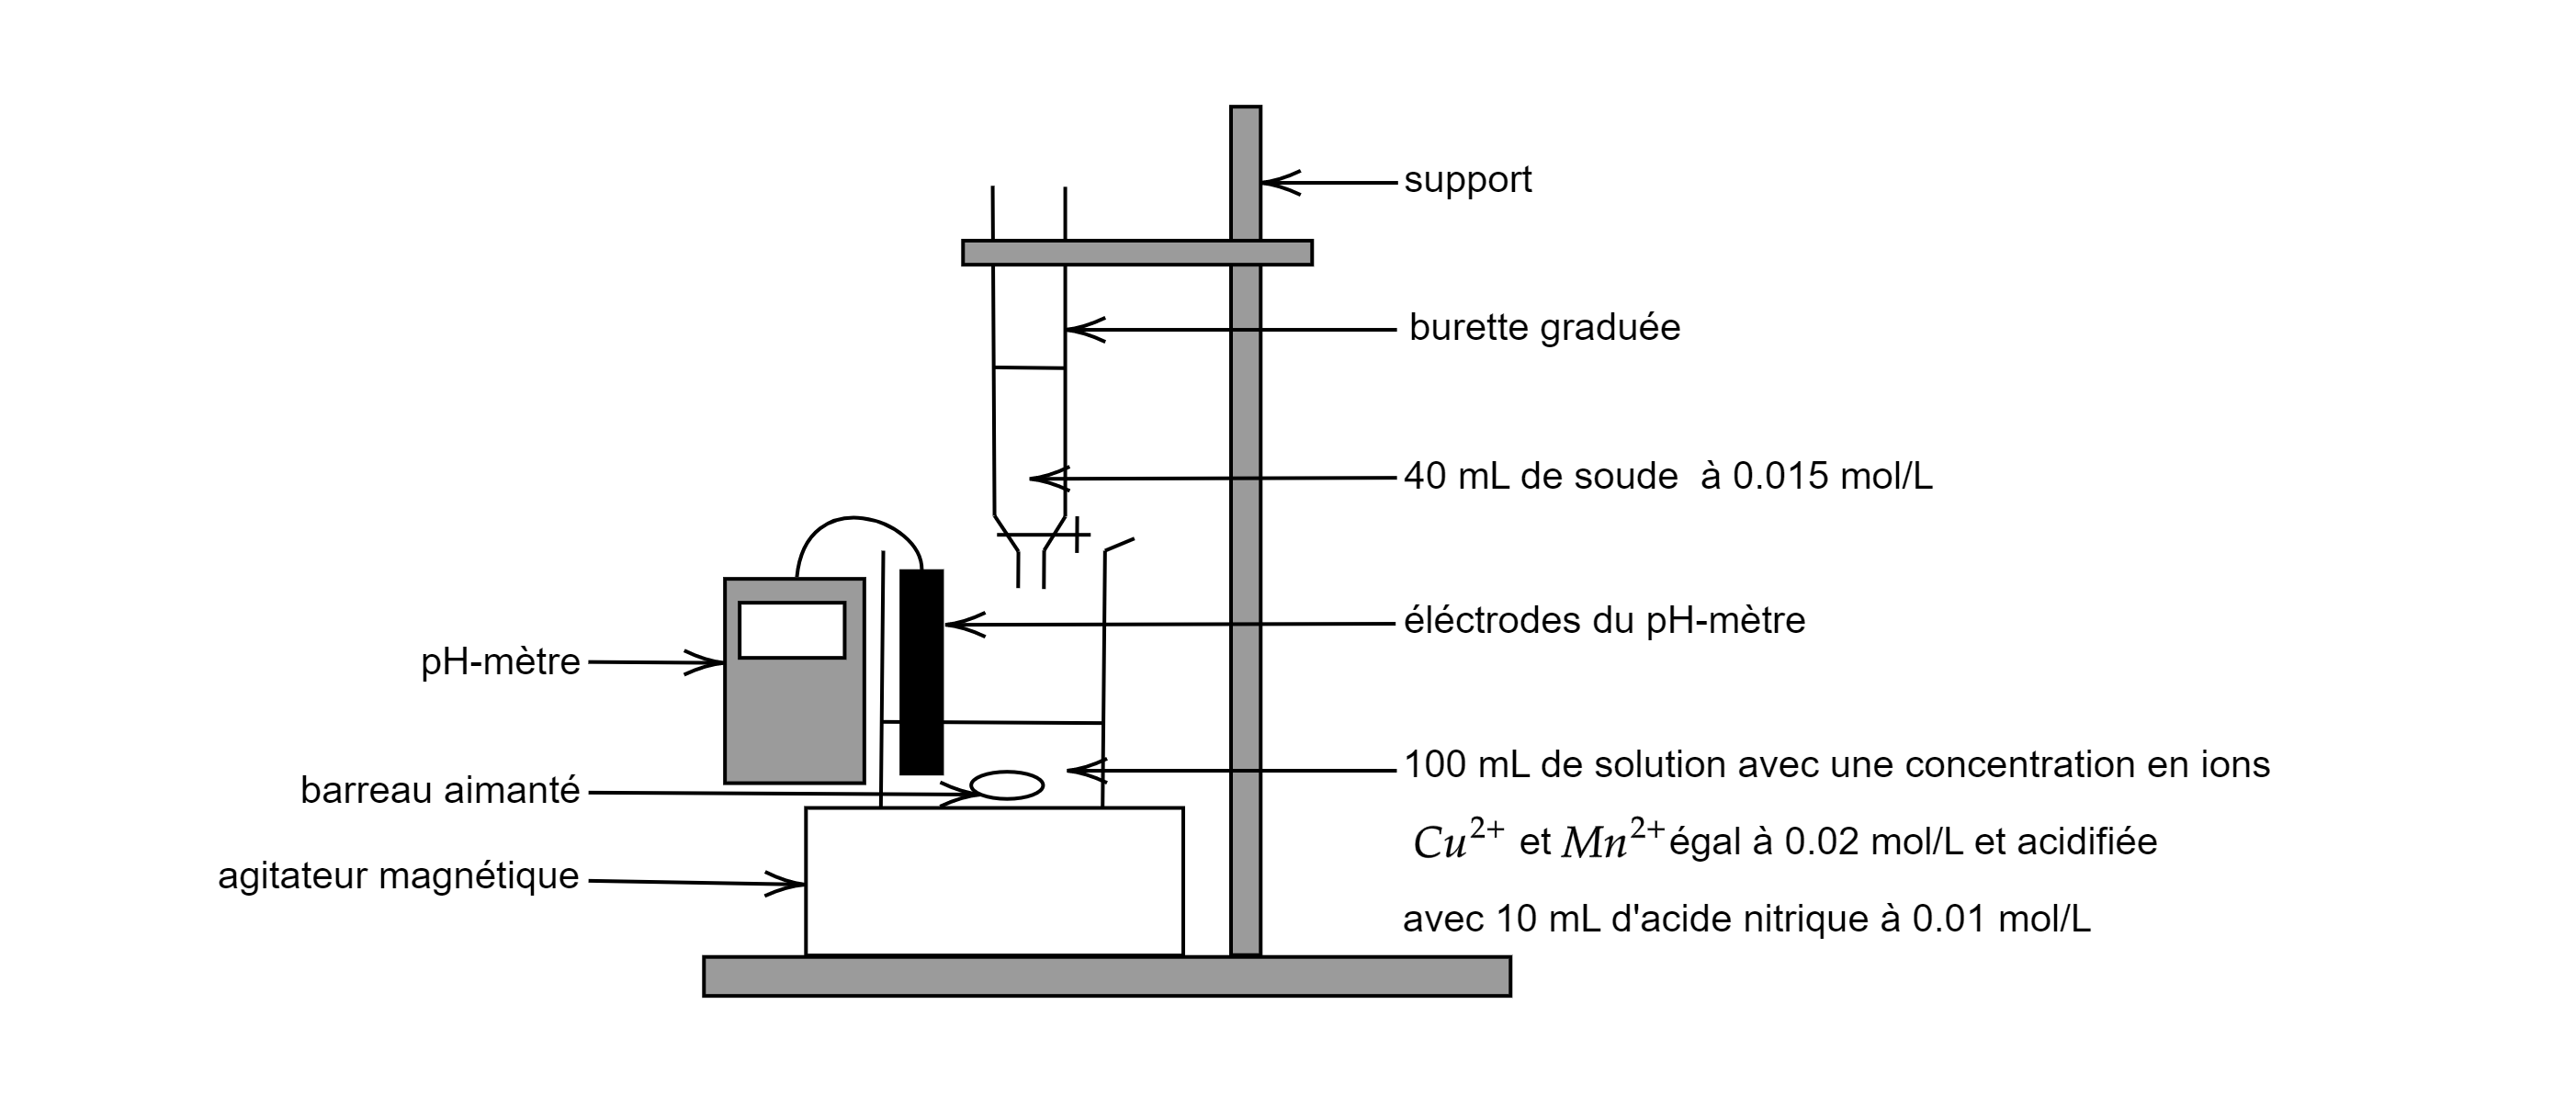
\includegraphics[scale=0.2]{Schema_dosage.png}
		\label{img:Schema_dosage}
		\caption{Schéma du montage expérimental du dosage des cations par de la soude}
	\end{center}
\end{figure}

On effectue une deuxième expérience où l'on pèse $m_{Cu} = 26 \pm 1$ mg de $Cu(NO_3)_2 \cdot 3 H_2O$ et $m_{Mn}= 20 \pm 1$ mg de $Mn(NO_3)_2\cdot 3 H_2O$. On transfère ces solides dans 2 béchers séparés où on verse environ 10 mL d'eau distillée. On rajoute ensuite dans chacun des béchers environ 10 mL d'une solution tampon de pH 6.5. 


\section{Résultats}
On trace la courbe du pH en fonction du volume de soude versé.
\begin{figure}[p]
	\begin{center}
		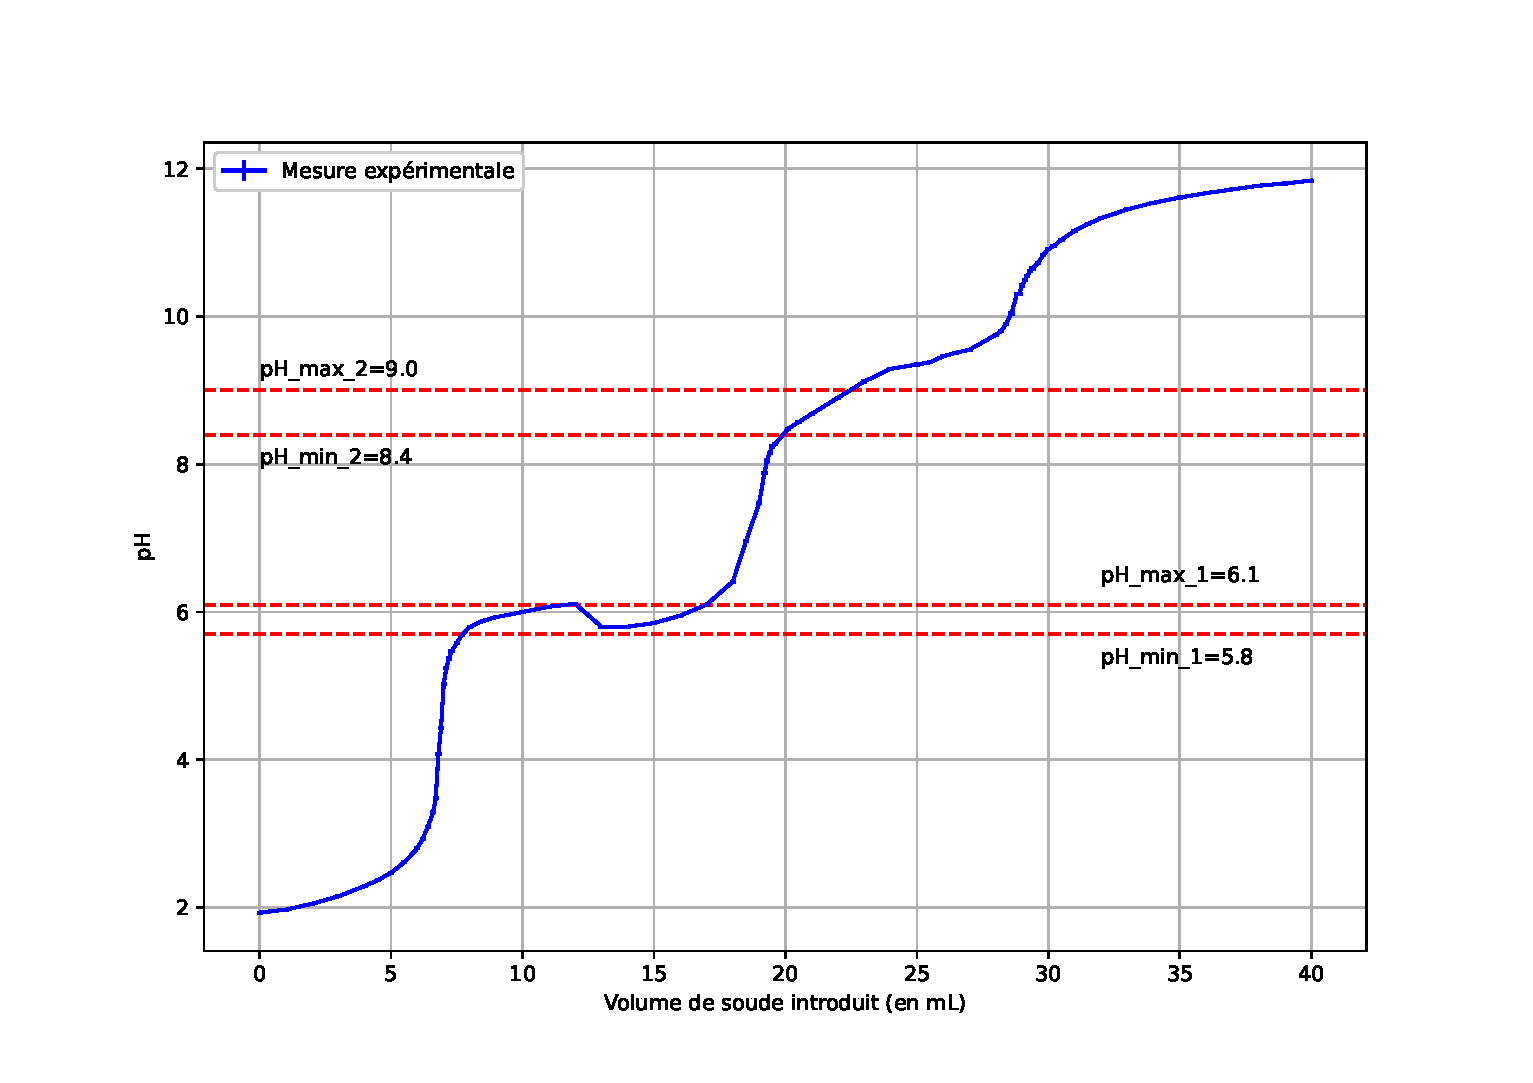
\includegraphics[angle=-90,scale=0.9]{Courbe_dosage.eps}
		\label{img:Courbe dosage}
		\caption{Courbe du pH en fonction du volume de soude versé}
	\end{center}
\end{figure}



On observe que la solution devient rapidement jaune, avant le premier saut de pH. On observe un précipité noir au début du saut de pH. Entre les deux sauts de pH la solution se trouble et prend une couleur verte.
On trouve un premier $pH_1$ de précipitation entre 5.8 et 6.1 et un deuxième $pH_2$ entre 8.5 et 9.3. La justification pour la détermination de ces pH est donnée dans la section suivante.

Pour la deuxième expérience on observe la formation d'un précipité blanc dans le bécher contenant les ions $Cu^{2+}$. La solution contenant des ions $Mn^{2+}$ se trouble mais on n'observe pas de précipitation. 

\section{Interprétation des observations et résultats}

Il y a principalement 3 réactions qui ont lieu lors du dosage. La réaction de précipitation de l'hydroxyde de cuivre(II):
\begin{equation}
Cu^{2+} + 2 H O^- \longrightarrow Cu(OH)_2
\end{equation}

La réaction de précipitation de l'hydroxyde de manganèse(II):
\begin{equation}
Mn^{2+} + 2 H O^- \longrightarrow Mn(OH)_2
\end{equation}

La dernière est la réaction de neutralisation de l'acide nitrique:
\begin{equation}
H_3 O^+ + H O^- \longrightarrow 2 H_20
\end{equation}

Le premier saut de pH est dû à la réaction de neutralisation entre l'acide nitrique et la soude, mais il est interrompu par la précipitation d'un premier hydroxyde. Le $pH_1$ en haut du saut est donc le pH de début de précipitation d'un hydroxyde. On utilise la même logique pour le deuxième saut de pH. La courbe de pH est censée être horizontale après le début de précipitation. Ce n'est pas le cas dans notre dosage, cela pourrait être dû au fait qu'on n'ait pas attendu assez longtemps après avoir ajouté la soude, ce qui fait que le pH n'a pas eût le temps de se stabiliser. On prend alors un pH minimum et un pH maximum pour avoir une incertitude sur les pH de précipitation. On détermine graphiquement ces pH en regardant les endroits sur les deux premiers sauts où le pH arrête d'augmenter rapidement.

On calcule donc:
\begin{align*}
pH_1&=\frac{pH_{max1}+pH_{min1}}{2} & \Delta pH_1 &= \frac{pH_{max1} - pH_{min1}}{2} \\
pH_1&=\frac{5.8+6.1}{2}=5.95 & \Delta pH_1 &= \frac{6.1- 5.8}{2}=0.15 \\
pH_2&=\frac{pH_{max2}+pH_{min2}}{2} & \Delta pH_2 &= \frac{pH_{max2} - pH_{min2}}{2} \\
pH_1&=\frac{9.0+8.4}{2}=8.4 & \Delta pH_2 &= \frac{9.0-8.4}{2}=0.3
\end{align*}
On a donc $pH_1=6.0 \pm 0.2$ et $pH_2=8.4 \pm 0.3$

On a observé que l'hydroxyde de cuivre(II) précipitait à un pH de 6.5 mais pas celui de manganèse. On en déduit donc que le $pH_1$ correspond au pH de début de précipitation de l'hydroxyde de cuivre(II).

Le troisième saut de pH nous donne l'équivalence entre un cation et la soude. La chute de pH vers 12 mL n'est pas expliqué par nos équations chimiques, l'ajout d'une base n'est pas censé diminuer le pH. Cela est peut-être dû à la formation d'un précipité qui se dépose sur les électrodes du pH-mètre, ce qui perturbe la mesure. 

On calcule la concentration en $Cu^{2+}$ et $Mn^{2+}$ dans la solution:
\begin{align*}
C_{Cu^{2+}}&=\frac{m_{Cu}}{M_{Cu(NO_3)_2 \cdot 3 H_2O} \times V} & C_{Mn^{2+}}&=\frac{m_{Mn}}{M_{Mn(NO_3)_2 \cdot 3 H_2O}\times V} 
\\
C_{Cu^{2+}}&= \frac{0.241}{241.60 \times 0.1} & C_{Mn^{2+}}&= \frac{0.214}{214.98\times 0.1}
\\C_{Cu^{2+}}&=9.975 \ mmol/L & C_{Mn^{2+}}&=9.996 \ mmol/L
\end{align*}
On calcule les incertitudes associées :
\begin{align*}
\Delta C_{Cu^{2+}}&= C_{Cu^{2+}}\times \left(\frac{\Delta m_{Cu}}{m_{Cu}} + \frac{\Delta V}{V} \right) & 
\Delta C_{Mn^{2+}}&= C_{Mn^{2+}}\times \left(\frac{\Delta m_{Mn}}{m_{Mn}} + \frac{\Delta V}{V} \right)
\\\
\Delta C_{Cu^{2+}}&= 9.975 \times \left((\frac{1}{241} + \frac{0.1}{100}\right) & 
\Delta C_{Mn^{2+}}&= 9.996 \times \left((\frac{1}{214} + \frac{0.1}{100}\right) \\
\Delta C_{Cu^{2+}}&= 0.05 \ mmol/L & \Delta C_{Mn^{2+}}&=0.06 \ mmol/L
\end{align*}
On a donc $C_{Cu^{2+}}=9.98 \pm 0.05$ mmol/L et $C_{Mn^{2+}}=1.00 \pm 0.06$ mmol/L. 

On utilise ensuite la relation qui relie le pH de début de précipitation au pKs: 
\begin{equation}
pH=pKe- \frac{1}{2}(pKs + \log C_0) \Longrightarrow pKs=2(pKe - pH)- \log(C_0)
\end{equation}

On calcule pour nos valeurs :
\begin{align*}
pKs_{Cu}&= 2(pKe-pH_1)-\log(C_{Cu^{2+}}) & pKs_{Mn}&= 2(pKe-pH_2)-\log(C_{Mn^{2+}}) \\
pKs_{Cu}&= 2(14-6)-\log(9.98\times 10^{-3})=18 & pKs_{Mn}&=2(14-8.4)-\log(1.00\times 10^{-2})=13.2
\end{align*}

Pour les incertitudes, on commence par calculer les incertitudes sur $\log(C_0)$:
\begin{align*}
	\Delta \log(C_0) = \left(\frac{\Delta C_0}{\ln(10)\times C_0} \right) \\
	\Delta \log(C_{Cu^{2+}})= \frac{0.05}{\ln(10)\times 9.98 }= 0.002 \\
	\Delta \log(C_{Mn^{2+}})= \frac{0.06}{\ln(10)\times 10 }= 0.003
\end{align*}

On peut maintenant calculer l'incertitude sur pKs :
\begin{align*}
\Delta pKs&= 2\times \Delta pH + \Delta log(C_0) \Longrightarrow\\
\Delta pKs_{Cu}&= 2 \times 0.2 + 0.002= 0.4 \\
\Delta pKs_{Mn}&= 2 \times 0.3 + 0.003 = 0.6
\end{align*}

\newpage
\section*{Conclusion}
Dans ce travail pratique on a déterminé le pKs de deux hydroxydes : $pKs_{Cu}=18\pm 0.4$ et $pKs_{Mn}=13.2\pm 0.6$. Cela semble cohérent avec le données trouvées \href{https://owl.oit.umass.edu/departments/Chemistry/appendix/ksp.html}{ici} annonce $pKs_{Cu}=18.8$ et $pKs{Mn}=13.3$.
 Nos incertitudes ne permettent pas d'expliquer la différence avec la valeur théorique. Nous avons peut-être sous estimé nos incertitudes, il faudrait refaire le dosage en attendant plus longtemps que le pH se stabilise et en ayant une agitation forte pour que le moins de précipité possible ne se dépose sur les électrodes. 



\end{document}